\documentclass[12pt]{article}
\usepackage{tikz}
\usetikzlibrary{arrows.meta}

\usepackage{amsmath}
\usepackage{physics}

\begin{document}

\section*{Analizo de fortoj por la eksperimento de Millikan}

\begin{center}
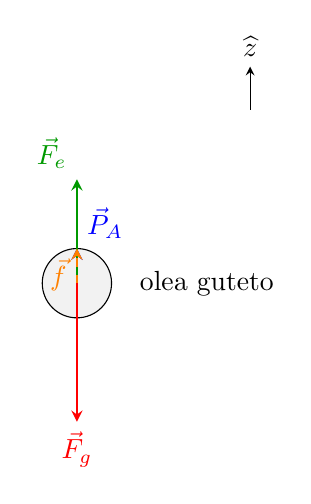
\begin{tikzpicture}[scale=1.1,>=stealth]

  % Akso z
  \draw[->] (2,2) -- (2,2.5) node[above] {$\widehat{z}$};

  % Guteto (olea guteto)
  \fill[gray!10] (0,0) circle (0.4);
  \draw (0,0) circle (0.4);
  \node at (1.5,0.0) {olea guteto};

  % Pezo (gravita forto) malsupren
  \draw[->,red,thick] (0,0) -- (0,-1.6)
    node[below] {$\vec{F}_g$};


  % Arkimeda forto supren
  \draw[->,blue,thick] (0,0) -- (0,0.4)
    node[above right] {$\vec{P}_A$};


  % Elektra forto (direkto laŭ E)
  \draw[->,green!60!black,thick] (0,0) -- (0,1.2)
    node[above left] {$\vec{F}_e$};


  % Aera frotado (nul por senmova guteto)
  \draw[->,orange,thick,dashed] (0,0) -- (0,0.4)
    node[below left] {$\vec{f}$};



\end{tikzpicture}
\end{center}

\end{document}
